\documentclass[10pt]{article}
\usepackage[margin=1in]{geometry}
\usepackage{mathptmx}
\usepackage[T1]{fontenc}
\usepackage[utf8]{inputenc}
\usepackage{microtype}
\usepackage{amsmath,amssymb}
\usepackage{booktabs}
\usepackage{graphicx}
\usepackage{float}
\usepackage{caption}
\usepackage{xcolor}
\usepackage{enumitem}
\usepackage{algorithm}
\usepackage{algpseudocode}
\usepackage[hidelinks]{hyperref}
\graphicspath{{evidence/}}

\title{\vspace{-1.4em}\Large Menu-Guided Classifier Agents for Minimum-Traffic Kernel Optimization:\\[2pt] \large Reaching the HBM Byte Floor on Levels 5--7}
\author{\normalsize Team 44 --- Hack the Chip (NYU $\times$ Annapurna Labs)\\[2pt]
\small Code and evidence: \url{https://github.com/SATYAPRAGNYA-KAR/trainium-agent-labs} (branch \texttt{minimum-traffic-agent})}
\date{\small October 10, 2026 --- all results simulator-verified; no device execution}

\begin{document}
\maketitle
\vspace{-2.2em}

\begin{abstract}
\noindent We study whether a small language model (Qwen3-8B) driving an agent loop can optimize NKI
matmul kernels to the HBM byte floor under a fail-closed checker, at levels 5--7 (worst-case byte
ratios $\leq 1.60$, $1.25$ and $1.05$ on four benchmark shapes). An unguided generation loop
produced \emph{zero} validated improvements in 90 attempts. Three changes produced the first
passes: (i) diagnosing failures \emph{behaviorally}, from hypotheses tested against the produced
numbers rather than error text; (ii) repairing the model's own near-misses instead of regenerating
from the correct-but-slow seed; and (iii) casting repair \emph{selection} as classification over a
fixed 15-option guidance menu --- each round the model chooses one guidance id and writes no code,
and a second call applies only that guidance's exact text. The loop produced one native kernel per
level that the official checker accepts at \emph{exactly} the floor ($1.00\times$ on all four
shapes, two evaluation seeds, CLI exit 0), plus verified $1.857\times$ intermediates. A robustness
suite over held-out aligned shapes ($9/9$), hostile value families ($20/20$) and ragged
non-divisible shapes ($0/9$) isolates partial-tile handling as the open failure. We also report the
negative results: from the clean $2.00\times$ seed the loop still fails, so the near-miss start is
load-bearing.
\end{abstract}

\section{Introduction}
Writing accelerator kernels is specialist work: the programmer decides which tiles move on-chip,
in which order, and how reuse is won. On memory-bound operations the objective is not arithmetic
speed but \emph{bytes}: every input element read once and the output written once defines a byte
floor, and a kernel's quality is its traffic ratio (bytes moved / floor). A wrong kernel does not
crash --- it returns plausible numbers --- so any optimization loop needs a checker that is as
strict about correctness as it is about speed.

This paper reports a one-day effort to drive such a loop with a small model under the
\texttt{nkibench} harness (NKI matmul, four benchmark shapes, levels 5--7 defined by tightening
traffic gates: $1.60\times$, $1.25\times$, $1.05\times$). The contributions are:
\begin{itemize}[leftmargin=1.4em,itemsep=1pt,topsep=2pt]
  \item a fail-closed checker with \emph{behavioral diagnosis} that names a fault from the numbers
        a kernel produces;
  \item \emph{near-miss-first repair}: restart from the model's own partially-correct attempts,
        which measurably beats regeneration from the seed;
  \item a \emph{menu-guided classify-then-apply} loop: repair selection is classification over a
        fixed authored menu, and generation is confined to executing the chosen change;
  \item formal per-level acceptance plus a robustness suite over declared held-out cases;
  \item honest negative results with byte-exact failure arithmetic.
\end{itemize}

\section{Task and Evaluation}
\textbf{Problem.} Produce an NKI kernel computing $C = A^{\top}B$ with \texttt{lhsT} of shape
$(K,M)$ and \texttt{rhs} of shape $(K,N)$, float32, for four shapes: $(128,128,512)$,
$(256,256,1024)$, $(512,128,512)$, $(256,512,1024)$. The shipped seed kernel is correct but wastes
up to $2.00\times$ the floor. \textbf{Metric.} The checker counts HBM bytes by instrumenting
\texttt{nisa.dma\_copy} during CPU simulation; ratio $=$ bytes / floor. \textbf{Acceptance} at a
level requires relative numerical error $\leq 2\cdot10^{-2}$ on every shape \emph{and} worst-case
ratio under the level gate. The gate is fail-closed: unmeasured traffic, inputs modified, or a
byte count \emph{below} the floor (impossible for a correct kernel) are failures, never wins.
Levels 5--7 share the four shapes and differ only in the gate ($1.60/1.25/1.05$); each level
checks through its own entry-point name, so formal evidence is a native kernel per level.

\section{System}
\subsection{Checker and behavioral diagnosis}
The acceptance decision is one function shared by the CLI and the agent loop: input mutation,
numerics (element-wise relative tolerance against a NumPy reference), then the traffic gate. When
numbers are wrong, the checker runs \emph{hypothesis tests on the produced output}: e.g.\ if the
candidate's matrix equals ``stationary-operand chunk 0 multiplied against every right chunk'', the
diagnosis states that the stationary operand never advanced past its first $k$-chunk. This
verdict-to-instruction translation matters: feeding raw verdicts back verbatim made the model
reproduce the same violation, a lesson this repository had already measured twice.

\subsection{Near-miss-first repair}
The unguided loop's failures are an asset. Across 90 unguided attempts (a pilot plus five frozen
repeats) no kernel was both correct and faster; the best \emph{correct} kernel remained the seed at
$2.00\times$. But many attempts \emph{did} find the byte-saving structure ($\approx1.86\times$)
while computing wrong numbers --- ``near-misses''. Repairing such a kernel is a small, local edit;
inventing the optimization from the seed is not. Every successful run reported here started from a
near-miss the model had authored itself.

\subsection{Menu-guided classify-then-apply}
Repair knowledge lives in a fixed menu of 15 options (stack an operand into a reused on-chip cache;
fix a stacked cache's width/stride; give the moving operand the symmetric treatment; keep the
contraction axis on the partition axis; split the K contraction; place tiles in the correct memory
region; match assignment shapes; hoist invariant loads; and a back-out control, among others).
Each option carries \emph{when} (the state that should trigger it --- the classifier's criteria)
and \emph{exact} (the complete change --- the applier's instruction). Algorithm~\ref{alg:loop}
shows the loop; Figure~\ref{fig:loop} shows it visually. The design follows the System-One split
of TypeSafe's Jev~\cite{jev}: a classifier owns the bounded choice, and a generative model only
executes the chosen action. Two properties make the loop measurable: every decision is logged
(state, chosen id, reason, self-reported confidence, both raw replies), and every choice is scored
against a deterministic \emph{expected guidance} derived from the same state by authored rules.

\begin{algorithm}[t]
\caption{Menu-guided repair loop (one run)}
\label{alg:loop}
\begin{algorithmic}[1]
\Require start kernel $k$; menu $M$ (15 options); round budget $R$; level gate $g$
\State $best \gets k$
\For{$r = 1$ \textbf{to} $R$}
  \State $e \gets \textsc{Evaluate}(k)$ \Comment{rules; numerics; traffic; seeds}
  \If{$e$ accepted at gate $g$} \State \Return $k$
  \EndIf
  \If{$\textsc{progress}(e) > \textsc{progress}(best)$} \State $best \gets k$ \EndIf
  \State $d \gets \textsc{Diagnose}(e)$ \Comment{hypothesis tests on produced numbers}
  \State $c \gets \textsc{Classifier}(e, d, M)$ \Comment{choose ONE guidance id; no code}
  \If{$c$ is the back-out control} \State $k \gets best$
  \Else \State $k \gets \textsc{Applier}(k, c)$ \Comment{apply only $c$'s exact text}
  \EndIf
\EndFor
\State \Return $best$
\end{algorithmic}
\end{algorithm}

\begin{figure}[t]
\centering
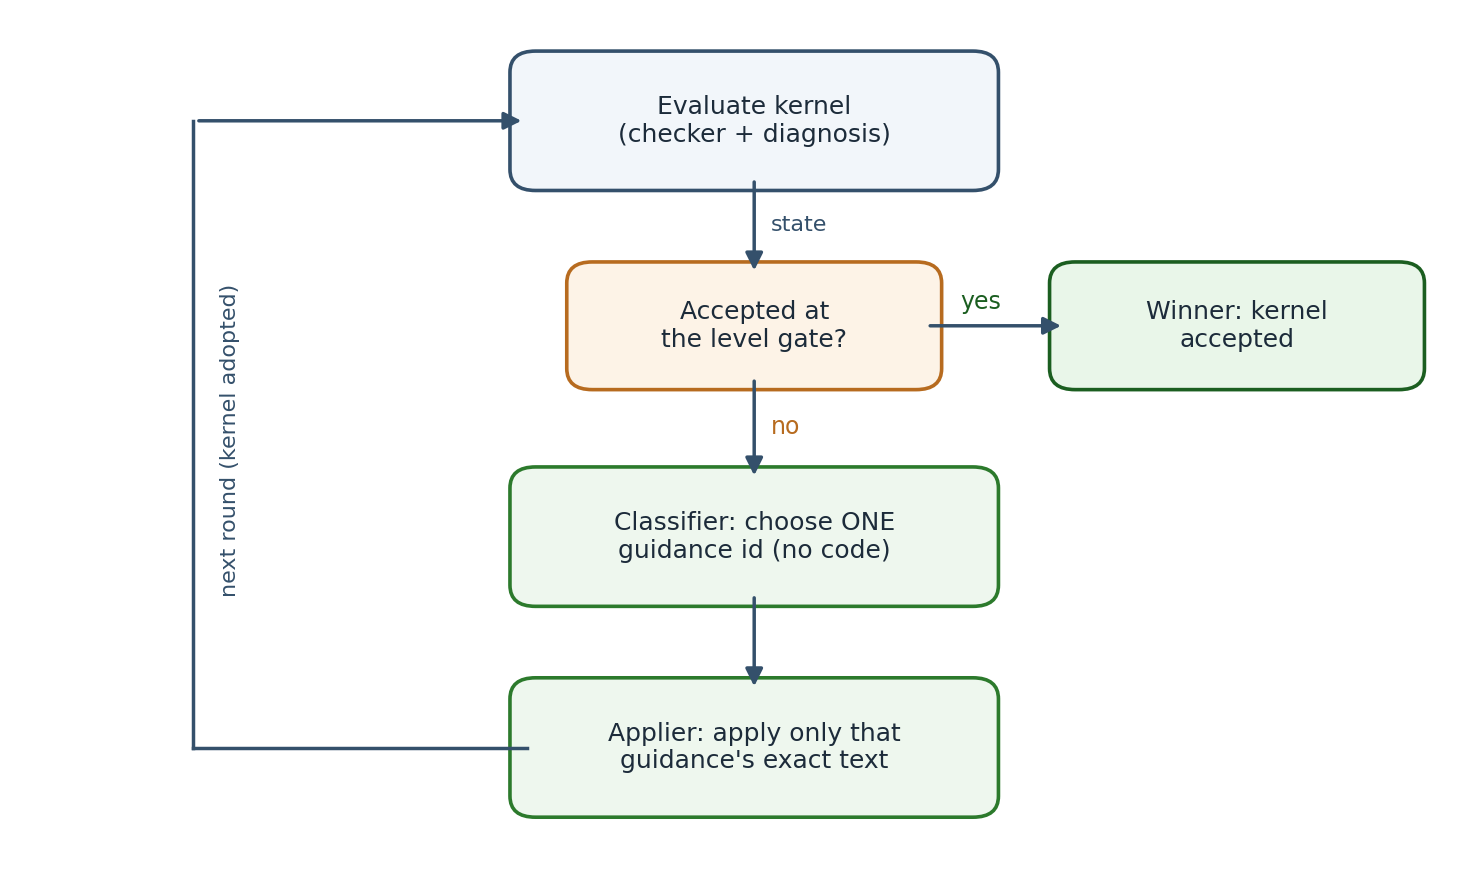
\includegraphics[width=0.86\textwidth]{loop_diagram.png}
\caption{The classify-then-apply loop. Selection is a bounded choice over a fixed menu; generation
is confined to applying the chosen change. The back-out control reloads the best kernel so a bad
choice costs one round, not the run.}
\label{fig:loop}
\end{figure}

\section{Experimental Protocol}
Model: Qwen3-8B served locally (vLLM, 8k context, thinking off). Environment: one cluster pod per
run; kernels evaluated by CPU simulation via \texttt{nki.simulate} (no device execution). Formal
acceptance: the official CLI (\texttt{nkibench.py --level L --check}) plus a structured evaluator,
at evaluation seeds 0 and 1. Robustness: a multi-process checker exercises the same algorithm on
the declared held-out cases --- aligned shapes at seeds $(17,29,43)$, five hostile value families
(zeros, negatives, repeated rows, sign-cancellation, large finite), and ragged shapes at seeds
$(7,11,23)$ --- 62 cases in total, judged by the same acceptance function. Runs: a pilot and five
frozen repeats unguided (90 attempts); line-guided surgical repairs; menu-guided runs from several
start states; and from-seed runs. The applier is near-deterministic, not deterministic; we report
demonstrations with their disclosures rather than rates.

\section{Results}
\subsection{Formal level acceptance}
Table~\ref{tab:levels} lists the verdicts. Each level has a native kernel accepted at exactly the
floor on all four shapes, at both seeds, with the CLI exiting 0. Table~\ref{tab:shapes} shows the
per-shape numbers. Two verified $1.857\times$ intermediates exist as well
(\texttt{agent\_kernel\_l6\_best\_1p86x.py}, \texttt{agent\_kernel\_verified\_1p86x.py}).
Figure~\ref{fig:levels} (left) plots seed vs.\ agent kernel against the three gates; (right) shows
classifier behaviour in the three solved runs: the level-5 run made three decisions with one
misfire absorbed by the back-out control; the level-6 floor landed on one disclosed retry; the
level-7 run matched the expected guidance $2/2$.

\begin{table}[H]
\centering
\caption{Formal verdicts. Each kernel is native to its level (entry-point name) and was verified
at evaluation seeds 0 and 1 with the official CLI (exit 0 on both).}
\label{tab:levels}
\small
\begin{tabular}{llrl}
\toprule
Level & Kernel (entry) & Worst & Acceptance \\
\midrule
5 & \texttt{menu\_guided\_1p00x} (\texttt{hoist\_load}) & $1.00\times$ & accepted, seeds 0/1 \\
6 & \texttt{l6\_nearmiss\_1p00x} (\texttt{block\_free\_dim}) & $1.00\times$ & accepted, seeds 0/1 \\
7 & \texttt{l7\_nearmiss\_1p00x} (\texttt{fully\_optimized}) & $1.00\times$ & accepted, seeds 0/1 \\
\bottomrule
\end{tabular}
\end{table}

\begin{table}[H]
\centering
\caption{Per-shape HBM bytes: the shipped seed vs.\ the agent kernel (identical across levels).}
\label{tab:shapes}
\small
\begin{tabular}{lrrr}
\toprule
Shape $(K,M,N)$ & Seed bytes (ratio) & Agent bytes (ratio) & Floor bytes \\
\midrule
$128,128,512$  & 589{,}824 ($1.00\times$) & 589{,}824 ($1.00\times$) & 589{,}824 \\
$256,256,1024$ & 3{,}670{,}016 ($1.56\times$) & 2{,}359{,}296 ($1.00\times$) & 2{,}359{,}296 \\
$512,128,512$  & 1{,}572{,}864 ($1.00\times$) & 1{,}572{,}864 ($1.00\times$) & 1{,}572{,}864 \\
$256,512,1024$ & 7{,}340{,}032 ($2.00\times$) & 3{,}670{,}016 ($1.00\times$) & 3{,}670{,}016 \\
\bottomrule
\end{tabular}
\end{table}

\begin{figure}[H]
\centering
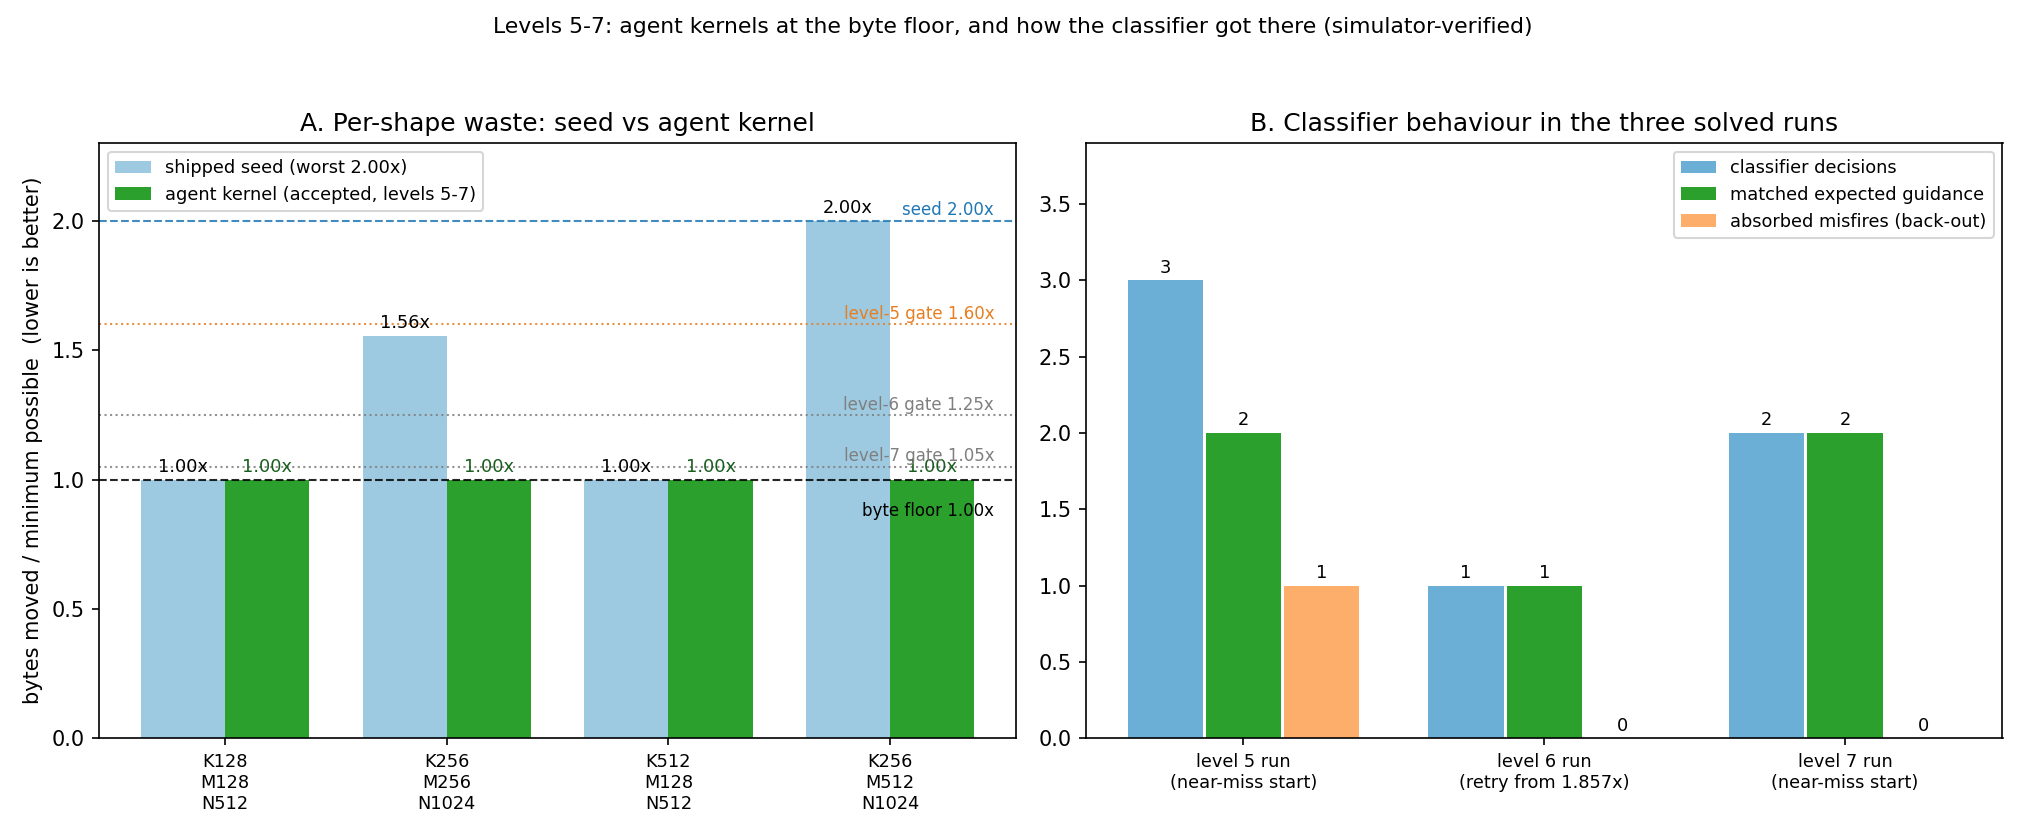
\includegraphics[width=0.92\textwidth]{levels_results.png}
\caption{Left: per-shape traffic ratio, seed vs.\ agent kernel, under the three level gates.
Right: classifier decisions in the three solved runs (one misfire absorbed by the back-out).}
\label{fig:levels}
\end{figure}

\section{Robustness}
Table~\ref{tab:robust} and Figure~\ref{fig:robust} summarize the robust check of the enclosed
algorithm. All 53 passing cases are correct \emph{and} within the level-5 bar; every failure is a
ragged (non-divisible) shape. The kernel assumes tile-multiple dimensions
($K/128$, $M/128$, $N/512$), so shapes such as $K{=}129$ or $N{=}513$ break it --- the
partial-final-tile trap the challenge document warns about. This is an honest open failure, not a
coverage gap.

\begin{table}[H]
\centering
\caption{Robust check (official checker internals, 62 cases).}
\label{tab:robust}
\small
\begin{tabular}{lrl}
\toprule
Case family & Passed & Note \\
\midrule
Optimization shapes, gates 5/6/7 & 24/24 & 4 shapes $\times$ 2 seeds $\times$ 3 gates \\
Held-out aligned shapes & 9/9 & seeds 17/29/43; never used for optimization \\
Hostile value families & 20/20 & 5 families $\times$ 4 shapes \\
Ragged non-divisible shapes & 0/9 & partial final tiles not handled \\
\bottomrule
\end{tabular}
\end{table}

\begin{figure}[H]
\centering
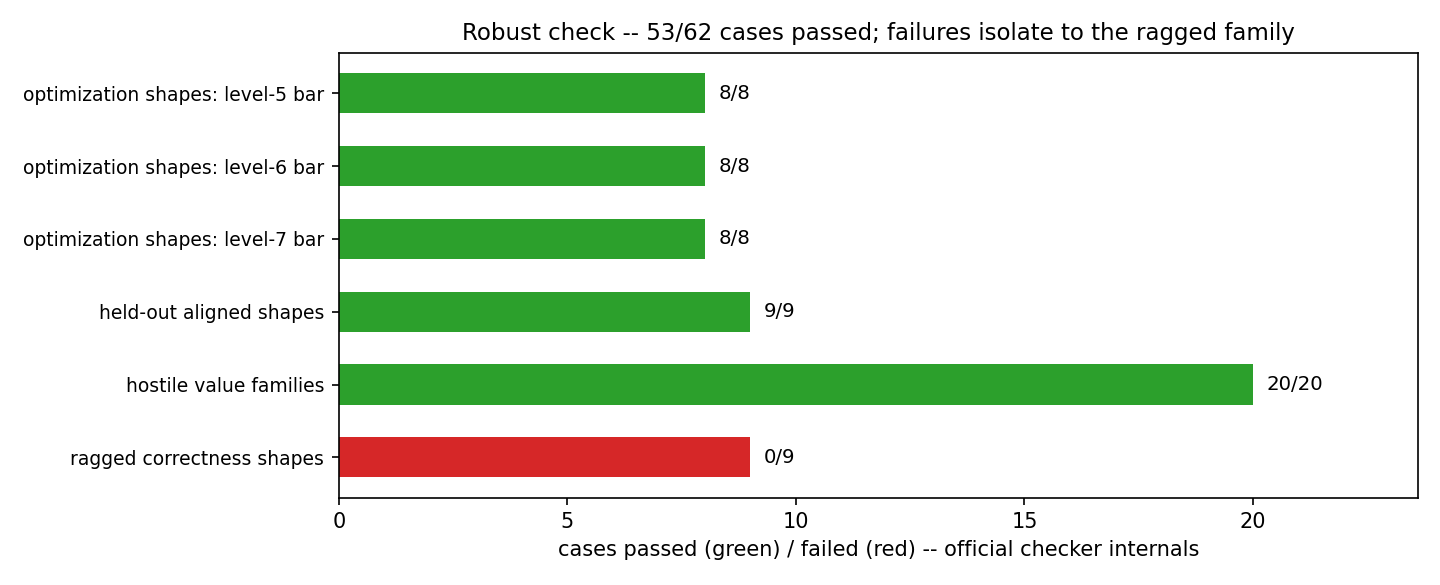
\includegraphics[width=0.80\textwidth]{robust_matrix.png}
\caption{Robustness by case family: 53/62 passed; the failures isolate to one declared family.}
\label{fig:robust}
\end{figure}

\section{Negative Results}
\textbf{From the clean seed.} Three formal runs started from the shipped $2.00\times$ seed
(renamed to each level's entry point) and all failed: the classifier chose the moving-operand
cache guidance, whose precondition --- an existing stationary-operand cache --- the seed does not
meet; the applier applied it anyway and broke the kernel (\texttt{UnboundLocalError}; once a
\texttt{gemm\_stationary\_fmax} overshoot); the classifier then misread the broken states as
``correct but too much traffic'' and repeated its choice. \textbf{Precondition-fixed retries.}
With explicit precondition text added to the menu, the applier added \emph{both} caches --- but
inside the output-tile loops, reloading both full operands per tile: traffic worsened to
$2.67\times$ and $4.00\times$, matching tile-count $\times$ full-operand arithmetic exactly, and
the classifier repeated its choice again. \textbf{Context slimming.} Removing the worked-example
block from the applier prompt was checked once and \emph{rejected}: without it the applier
misapplied the guidance and the loop stalled, so the block stayed. \textbf{Smaller failures.} One
classifier misfire on a gate-only state (absorbed by the back-out, one round lost); one applier
overshoot on a restacked start, showing selection and application can fail independently.

\section{Limitations and Threats to Validity}
\begin{itemize}[leftmargin=1.4em,itemsep=1pt,topsep=2pt]
  \item \textbf{Near-miss dependence.} The loop repairs structures the model has already found;
        from the clean seed it has not produced even a below-$2.00\times$ result.
  \item \textbf{Ragged shapes fail} ($0/9$); partial-tile handling is open.
  \item \textbf{Authored knowledge.} Menu texts, the worked example, and the expected-guidance
        rules are team-authored; selection and application are model-driven. Per-round logs expose
        every choice, so the boundary is auditable.
  \item \textbf{Simulator only}, single runs per configuration (near-deterministic applier; the
        level-6 floor landed on a disclosed retry). Self-reported confidences are uncalibrated.
  \item \textbf{Scope.} Four benchmark shapes plus declared held-outs; no device timing
        (latency is out of scope here).
\end{itemize}

\section{Related Work}
The problems this loop solved are verifier-first agent design problems: constraints belong in the
checker, and a verdict must be translated into a named change~\cite{challenge}. The classify-then-
apply split follows the System-One model class proposed by TypeSafe (``Jev''), where bounded
choices are made by a classifier and generation is reserved for executing the chosen
action~\cite{jev}. Using a fixed authored action menu with the model as selector is closely
related to experience-driven guideline selection in tool-using agents; we did not survey that
literature formally, and the contribution here is empirical: measured effects of near-miss-first
repair and menu-guided selection under a fail-closed checker.

\section{Conclusion}
A small model reached the HBM byte floor on levels 5--7 --- native kernels, two seeds, official
checker, exit 0 --- not by generating better kernels but by (i)~seeing its own near-misses as the
starting point, (ii)~receiving behavioral diagnoses instead of verdicts, and (iii)~choosing among
authored repairs as a classifier while generation only executes the choice. The negative results
are equally load-bearing: from the clean seed the same loop fails, and the ragged shapes expose a
real, named gap. We report both. All decisions, replies and evaluations are logged in the
repository's evidence folder~\cite{evidence}.

\begin{thebibliography}{2}\small
\bibitem{challenge} \textit{CHALLENGE-kernel-agent.md} (this repository): measured lessons on
verifier-first loops. \url{https://github.com/SATYAPRAGNYA-KAR/trainium-agent-labs/blob/master/projects/02-kernel-agent/CHALLENGE-kernel-agent.md}
\bibitem{jev} TypeSafe AI, ``Introducing System One Models \& Jev,'' Sep 2026.
\url{https://typesafe.ai/blog/introducing-system-one-models-and-jev}
\bibitem{evidence} Full evidence trail: \texttt{evidence/FORMAL-CHECK.md},
\texttt{evidence/GUIDANCE-CLASSIFIER.md}, \texttt{evidence/ERROR-CATALOG.md}, and per-round logs
(\texttt{evidence/*rounds.jsonl}) in this repository.
\end{thebibliography}

\end{document}
